\chapter{Développement de modèles}

\section{Interaction sociales}
Ne pas présenter sous cette forme

Les interactions sociales ont lieu d'une part pour modifier les activités car certaines peuvent être partagées, comme regarder la télévision. D'autre part ces interactions peuvent également modifier les actions réalisées sur des systèmes, comme l'ouverture des fenêtres.

Le développement des modèles suivant s'intéressera également aux dynamiques sociales entre les occupants. L'influence de la famille ou des colocataires en terme de négociation et de régulation sera en outre étudiée.

Plessis et al. \cite{Plessis-14} introduisent la notion de confort du groupe qui est utilisée pour déterminer quel action le groupe choisi (ex: augmenter la température, ouvrir la fenêtre). En opposition aux actions individuels (adaptation de l'habillement, changement d'activité).

\subsection{Quantification des activités}

Dans le but de quantifier les activités, on défini une unité appelée unité de service. Cette unité est définie par occupant. L'unité de service d'un logement ou d'une zone pour une activité peut donc être déterminé par l'agrégation de l'unité de service pour tous les occupants du logement. Cette agrégation dépend de la nature des activités, elle peut être partagée ou additive.

Une nature d'activité partagée correspond à une activité réalisée ou profitant à deux occupants ou plus. Par exemple, l'activité regarder la TV est considérée comme partagée car plusieurs occupants peuvent profiter de la même unité de service. Une activité est dite additive si l'unité de service du logement est la somme des unités de service individuelle. Par exemple, l'activité de toilette corporelle est additive car réalisée seule. Le tableau \ref{tab:activité et unité de service} présente les unités de services et la nature des activités. Une activité partagée signifie quelle peut être partagé ou additive.

\begin{table} [H]
\centering
\begin{tabular}{|l|l|l|}
\hline
Activité & Unité de service & Nature de l'activité \\
\hline
Dormir & Durée & Partagée \\
Passif & Durée & Additif \\
Audio-visuel & Durée & Partagée \\
Bureautique & Durée & Additif \\
Cuisine & Durée/intensité & Partagée \\
Nettoyage & Surface & Additive \\
Toilette corporelle & Nombre de douche & Additive \\
Vaisselle & Quantité de vaisselle & Partagée \\
Bricolage & Durée & Additive \\
\hline
\end{tabular}
\normalsize
\caption{Nature d'activité et unité de service}
\label{tab:activité et unité de service}
\end{table}

\section{Activités et présence}

\subsection{Bureaux}

\subsection{Logements}

\section{Gestion des ouvrants}

1- Etat de l'art des modèles de gestion des fenêtres. Etudes sociologiques sur l'ouverture des fenêtres. Vérification du modèle utilisé par Schweiker et al. \cite{Scweiker-12}

2- Présentation du modèle courant 

3- Incorporation de phénomènes sociologiques qualitatifs au modèle:
    - Lorsque l'activité cuisine a lieu on ouvre la fenêtre
    - Lorsque l'occupant se réveille alors il ouvre la fenêtre
    
\section{Gestion des stores}

1- Etat de l'art sur les drivers de la gestion des stores

2- Présentation du modèle courant

3- Incorporation de phénomènes sociologiques qualitatifs au modèle:
	- Lorsque l'activité audio-visuelle a lieu on ferme les stores
	- Lorsque l'activité dormir a lieu on ferme les stores
	
\section{Gestion de l'éclairage}

1- Présentation du modèle courant

2- Incorporation de phénomènes sociologiques qualitatifs au modèle:
	- Lorsque l'activité audio-visuelle a lieu on ferme la lumière
	- Lorsque l'activité dormir a lieu on éteins forcément la lumière

\section{Utilisation des appareils électriques}

\subsection{Types d'appareils électriques}

Widén (2009) a catégorisé les appareils électriques en fonction de l'utilisation de la puissance:
\begin{table} [H]
\centering
\begin{tabular}{l|l}
Type de puissance & Exemple \\
\hline
Puissance non définie par l'activité & Appareils de froid, radio réveil \\
Puissance constante pendant l'activité & Télévision, Appareils de cuisson \\
Puissance constante après l'activité & Machine à laver, lave vaisselle \\
Puissance constante après avec contrainte de temps & Bains, douches \\
Activité avec puissance dépendante du temps & Éclairage (variations journalières et de saison) \\
\end{tabular}
\end{table}
Une catégorisation de la sorte permet une étude temporelle de la variation d'énergie.

\subsection{Modélisation de la possession et de l'utilisation des appareils électriques}

Jaboob (2015) propose une modélisation du taux de pénétration \footnote{Le taux de pénétration aussi appelé taux d'équipement est le pourcentage de la population équipée d'un appareil électrique}de la possession, de l'utilisation et de la fraction de puissance des appareils électriques. Cette modélisation est de type bottom-up pour chaque famille d'appareil, cela permet de considérer la diversité des ménages, des comportements individuels des occupants et bien sûr les caractéristiques intrinsèques des appareils. La modélisation de la possession des appareils est réalisée par régression logistique. La modélisation de l'utilisation des appareils considère d'une part l'allumage et d'autre part sa durée d'utilisation. L'allumage est modélisé par Bernoulli et la durée par un processus aléatoire à temps continu. La modélisation de la fraction de la puissance est réalisée par processus de Bernoulli ou de Markov.

\section{Gestion des consignes de température}

1- Que cherche t-on? Prédire la température de consigne pour l'envoyer au cœur de calcul.

2- Introduction sur le choix de la température de chauffage (Brisepierre]

3- Comment la température de consigne est utilisée par EnergyPlus? En étudiant la température intérieure on s'aperçoit qu'elle est strictement égale à la température de consigne. Hypothèse également faite par le CEREMA dans ces travaux sur le suivi de bâtiments démonstrateurs à basse consommation. (p127  Bat démonstrateurs à basse consommation d'énergie - Enseignements opérationnels tirés de 60 constructions et rénovations du programme PREBAT 2012-2015). "L'analyse statistique des températures en période de chauffe permet d'estimer la température en hiver en se basant sur la mesure de la température intérieur pendant les heures de fonctionnement du chauffage et pendant les heures d'occupation identifiées par enquête."

4- Quels sont les facteurs influençant l'utilisation des systèmes de chauffage.

Comparaison des études paramétriques des déterminants de la température de chauffage adoptée par les ménages (CGDD, INRA, INSEE, CREDOC, Annex53, Kelly, Andersen)

Notre choix se porte sur le modèle de Kelly et al. car il est basé sur une étude significative, car ...

5- Choix pour le modèle de Kelly. Avec adaptation pour un modèle plus parcimonieux.

Pour développer un modèle, de type régression linéaire multiple, un logiciel de programmation statistique - comme R - a été utilisé. Ce type de logiciel permet de déterminer les coefficients Alpha et $a_{i}$ de l'équation de régression:

\begin{equation}
T_{int} = Alpha + \sum\limits_{i=1}^n a_{i} * V_{i} 
\end{equation}

Avec $T_{int}$ la température intérieure journalière, $Alpha$ et $a_{i}$ les coefficients à déterminer pour la régression et $V_{i}$ les valeurs des variables explicatives.

Pour obtenir les différents coefficients sous R il suffit de rentrer la fonction lm() en y spécifiant la variable à expliquer, les variables explicatives et la localisation du fichier:
\begin{verbatim}
   lm(Tint ~ Text + Text2 + Localisation + ... + Dbl_Glz + Wall_U, data = mydata)
\end{verbatim}

Le logiciel R génère alors les coefficients de la régression et 

Au risque de 1\%, il n'existe pas d'association statistiquement significative entre la température intérieure et les variables explicatives: déclaration de température de consigne, présence d'un programmateur automatique, tranche d'age de 60-64 ans, présence d'un système de chauffage central et d'un système de chauffage au gaz d'appoint. Ces variables explicatives sont donc supprimées du modèle développé.

Nous proposons aussi dans le fichier de configuration de laisser la possibilité aux utilisateurs de ne pas définir certains paramètres lorsqu'ils ne sont pas connus!

6- Variation journalière



7- Interactions sociales ...

Le modèle de base de Kelly peut être complété par l'incorporation d'informations qualitatives supplémentaires

La température de consigne fixée à 19 \degre C depuis le choc pétrolier de 1974 fait figure de norme mais ne reflète pas les faits réels. Son influence sur les consommations énergétiques y est très fortement corrélé et un ajustement plus fidèle à la réalité est nécessaire.
Pour cela le modèle proposé consiste à tirer sur une loi normale la température de base issue du bureau d'études d'Enertech. Puis, en fonction des paramètres d'influences V (age, genre, charge financière, zone, longue absence...) la base est modifiée:

\[T_{consprinc}=T_{base}+\sum_{V}X_{V}\]

Cette approche proposée par Vorger \cite{Vorger-14} est très souple et permet notamment de gérer les réduits. Son calibrage est néanmoins discutable car basé sur le bon sens. En ce basant sur le \textit{British Home Heating Study} qui a réalisé une enquête sur les systèmes de chauffage et de contrôle, un modèle sur le choix de la température de consigne, notamment en fonction du systèmes, peut être créé plus finement. Cette enquête est composée d'un questionnaire et de mesures dynamiques (températures, humidité relative, ...) sur un échantillon de 32 familles anglaises.

La récupération de ces données devrait se faire par l'intermédiaire de l'Université de Nottingham...

\section{Consommations d'eau chaude sanitaire}

\subsection{Systèmes}

Le modèle d'ETI ainsi que des données nationales (A trouver INSEE) peut permettre de modéliser les systèmes de chauffage de l'eau et le taux de pénétration des systèmes. Cette modélisation préalable est souvent omise dans les modèles de puisages d'ECS alors que son impacte sur les consommations finales en dépend relativement significativement.

On recense trois principales énergies pour la production d'eau chaude sanitaire: le gaz, l'électricité et les énergies renouvelables. Les chauffes-eau au gaz et électriques sont soit instantanés soit à accumulation. Concernant les énergies renouvelables, on retrouve de manière croissante le ballon thermodynamique ou pompe à chaleur et le chauffe eau solaire d'appoint.

\subsection{Volumes de consommation}

Selon Evarts et Swan \cite{Evarts-13} les puisages d'ECS sont très diverses selon les ménages et donc dépendent de leurs caractéristiques socio-démographiques. La fréquence et l'intensité des puisages sont encore plus fortement corrélés aux activités des occupants.

Selon les activités en cours, des puisages d'ECS y sont associés. A titre d'exemple, l'activité nettoyage corporelle implique un puisage en lien avec celui de la douche ou du bain.

L'ADEME a lancé un programme de recherche, baptisé PACTE, pour améliorer l'efficacité énergétique de l'ECS dans l'habitat. Ces travaux visent à améliorer la prise en compte de la dimension socio-comportementale de l'usage de l'ECS et à modéliser, simuler et évaluer le fonctionnement des équipements. La figure \ref{fig:PACTEECS} présente les partenaires du PACTE ECS, dont l'investissement est de plus 8 millions d'euros sur 5 ans.

\begin{figure}[h]
\centering
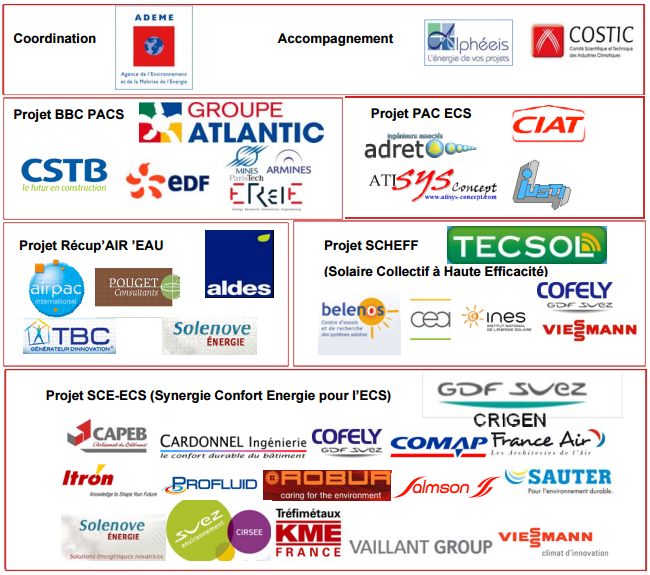
\includegraphics[scale=0.8]{Images/PACTEECS}
\caption{Les différents partenaires du PACTE ECS}
\label{fig:PACTEECS}
\end{figure}

La figure \ref{fig:Foisonnement_ECS} révèle la diversité de consommation à l'échelle du logement plutôt qu'à celle d'un immeuble.

\begin{figure}[h]
\centering
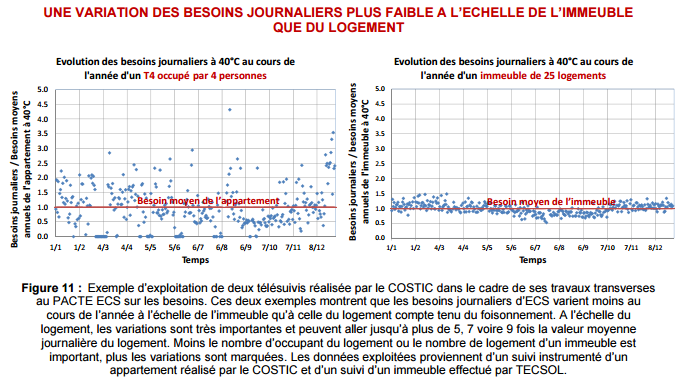
\includegraphics[scale=0.9]{Images/Foisonnement_ECS}
\caption{Importance de l'information à l'échelle du logement pour prendre en compte la diversité des consommations}
\label{fig:Foisonnement_ECS}
\end{figure}

La publication ADEME-COSTIC des résultats valorisés est prévue courant 2016 alors que l'étude se tient depuis 2011.

Contacter le directeur technique de COSTIC: Cedric Beaumont (prestations@costic.com) pour récupérer les résultats non agrégés 
